\chapter{Random Numbers}\label{ch:random-numbers}


Suppose that many identical systems are in the identical conditions and a physical quantity is measured in each system, we tend to think that the outcomes are also identical since the conditions uniquely determine the outcomes.  Newton's equations, Maxwell's equations, many other laws of physics are deterministic.  There is no room for uncertainty. Of course, that view is unrealistic in the real world.  All experimental data contain error bars due to noise. Not only the experimental data, quantum mechanics and statistical mechanics assume that the physical quantities are stochastic at the fundamental level.  The quantities do not have a unique value and fluctuate from measurement to measurement even when the condition is exactly the same.  In this chapter, we consider how to realize such a stochastic quantity in digital computers.  Since computers are completely deterministic, it looks impossible to deal with stochastic quantities.  However, there are ways to calculate stochastic quantities using \textit{random numbers}. 
In physics,  many stochastic processes are simulated on computers using random numbers.  Such methods are called Monte Carlo simulation after the famous casino city Monte Carlo in Monaco.  Understanding the random numbers is very important for computational physics.

Actually, random numbers are already used by the computers even at the system level and generating good random numbers is a serious issue for data security (encryption) in modern information technology.  Therefore, stochastic variables are not new to the deterministic digital computers.

\noindent
\section{Stochastic Variables}

A regular variable $x$ holds a certain value assigned to it and the value remains the same until a different value is assigned.  For example, the position of a particle at a certain time is uniquely determined by an initial condition and there is no uncertainty with it.  It is said that the trajectory is fully deterministic.  However, the trajectory is not always deterministic.  In real world, the environment may apply noisy forces on the particle.  In such cases the trajectories of the particles starting with the same initial conditions may take different trajectories. Then, the position of the particle cannot be expressed as a regular variable.  Instead it is a stochastic variable $\hat{X}$.  The stochastic variable does not holds a certain value.  When we try to retrieve the value from the stochastic variable, it picks a number from a so-called sample space with a certain probability assigned to that number.

For example, the number $\hat{X}$ obtained by rolling a die is a stochastic variable.  When the die is rolled  one number is obtained out of the sample space $\{1, 2, 3, 4, 5, 6\}$ and the probability to get the number is $1/6$.   In general, a discrete stochastic variable $\hat{X}$ is defined with an sample space $\{ x_i, i=1, \cdots, N\}$ and the corresponding probability $P_i$.  Note that the probability must satisfy $P_i \geq 0$ and $\sum_i P_i=1$.

A stochastic variable is fully characterized by the sample space and the probability distribution. 
We often characterize it with a few statistical quantities, namely the mean value $\mean{x}$ and variance $\Delta x$ defined by  
\begin{subequations}
\begin{eqnarray}
\mean{x} &=& \sum_i x_i P_i \\
\Delta x &=& \sqrt{(\mean{x - \mean{x})^2}} = \mean{x^2} -\mean{x}^2\, .
\end{eqnarray}
\end{subequations}
Although these two quantities alone cannot fully describe the stochastic variable, they usually give us a reasonable picture of the variable.

Similarly, a continuous stochastic variable is defined with a sample space $\{ a < x < b \}$. The probability to find a value between $c$ and $d$ is expressed with a probability density $\rho(x)$ as
\begin{equation}
P(c<x<d) = \int_c^d \rho(x)\, \md x
\end{equation}
The density must satisfy $\rho(x) \geq 0$ and $\int_a^b \rho(x)\, \md x = 1$ (normalization).  
The mean is defined by
\begin{equation}
\mean{x} = \int_a^b x \rho(x) \md x
\end{equation}
For example, a normally-distributed stochastic variable $\hat{X}$ is defined with the sample space $\{-\infty < x < \infty\}$ and $\rho(x) = \displaystyle\frac{\sigma}{\sqrt{2\pi}} \me^{-x^2/2\sigma^2}$.  Its mean and variance is $\mean{x}=0$ and $\Delta x = \sigma$.

A question is  how to realize the stochastic variable in computers. That is the main topics in this chapter. 

\noindent
\section{Uniform Random Numbers}


\begin{figure}
	\centering
	\begin{subfigure}{0.45\textwidth}
		\centering
		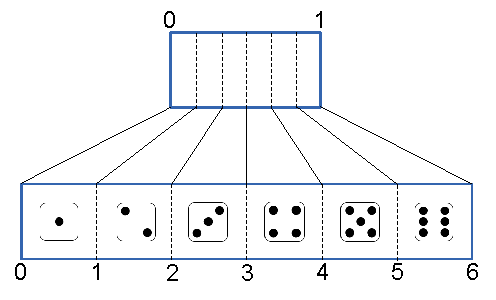
\includegraphics[width=2.5in]{15.Random-Numbers/map2die.pdf}
		\caption{Mapping from random numbers uniformly distributed between 0 and 1 to discrete random numbers.}
		\label{fig:map2die}
	\end{subfigure}
	\begin{subfigure}{0.45\textwidth}
		\centering
		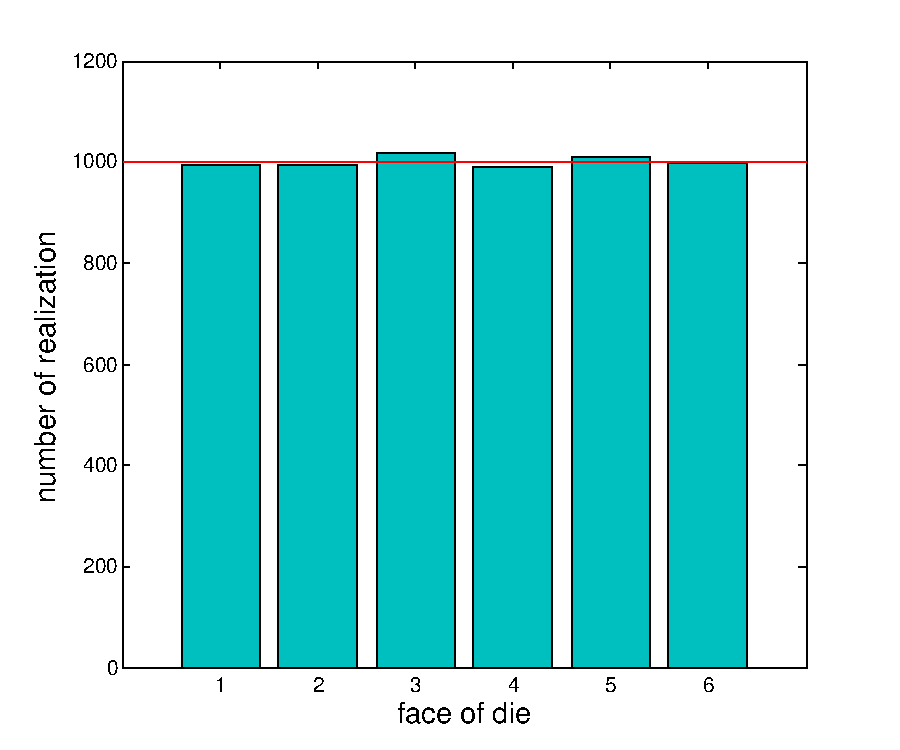
\includegraphics[width=2.5in]{15.Random-Numbers/virtual_die.pdf}
\caption{Statistics of the virtual die.  Due to the finite number of realizations, the probability is close but not exactly uniform.}
\label{fig:die_stat}
	\end{subfigure}
\caption{Virtual Die}\label{fig:virtual_die}
\end{figure}

We begin with a standard stochastic variable $\hat{R}$ with the sample space $\{ 0 \le r \le 1\}$ with uniform distribution $\rho(r)=1$. In computer, $\hat{R}$ is a random number generator.  Upon request, it generates a number $r$ between 0 and 1 at random.  At each call, we get a different value which has no relation to the previous values. Once we have $\hat{R}$,
we can construct random numbers with other kind of distributions by mathematical transformation as discussed below.  Therefore, we first investigate the basic uniform random number generators.  The uniform random number between 0 and 1 has the mean value $\mean{r}=1/2$ and the variance $\sigma=\mean{(r-\mean{r})^2}=1/12$.

All variables used in computer programs are deterministic and no room for uncertainty.  Then, how can we generate a random number?  The answer is No. We can't generate true random numbers by computer program.  However, there are procedures which generate deterministic sequences of numbers that look like random numbers.  They are called pseudo random numbers.  In most applications in physics, the pseudo random numbers are good enough when they are used with a certain care.  There are many algorithms to generate the pseudo random numbers.  A most popular method, known as linear congruential generator,  generates a sequence of random numbers $I_i$ by a recursive equation
\begin{equation}\label{eq:rand}
I_{i+1} = a\, I_i + b\quad \text{mod } c
\end{equation}
where $a$, $b$, and $c$ are integer constants. Then, the random number $r_i = I_i/c$ is a pseudo random number in the range of $0<r_i<1$. 
The most of the random generators supplied by computer systems are based on this algorithm.  In MATLAB, \texttt{rand()} generates random numbers between 0 and 1.
 
The quality of the random number depends on the choice of $a$, $b$, $c$.  Note that total number of possible random numbers are limited to $c$ at the best.  This type of pseudo random numbers are periodic and after a certain iterations the same sequence comes back. The longest possible period is $c$. It has been shown that a set of parameters $a=7^5=16807$, $b=0$, and $c=2^{31}-1=2147483647$ provides excellent uniform random numbers with the maximum periodicity $2^{31}-1$.
 
The recursive equation (\ref{eq:rand}) must start with a certain initial number $I_0$ called ''seed''. If you do not specify a seed, a fixed default seed is used and the same sequence of random numbers is obtained every time.  In order to avoid the use of the same random numbers, we must pick a different seed every time. For example, you can use the current date and time to reset the seed.  In MATLAB, \texttt{rng('shuffle')} does it.

 
\begin{example}[A Virtual Die]

\medskip
\noindent
We make a virtual die based on the congruential generator.  The uniform random numbers between 0 and 1 is mapped to integer random numbers between 1 and 6.
First, we generate a basic uniform random number $r$ and multiply 6 to it.  If $N-1 < 6 r \leq N \,( N=1,\cdots, 6)$, then the die gives the value $N$. For example, if the random number is $r=0.19$, then, $6r= 1.14$.  This corresponds to $2$ on the die. Figure \ref{fig:map2die} illustrates the mapping from the uniform random number to the die. Program \ref{prog:virtual_die}, we roll the virtual die 6000 times. If the die is far, each face is realized 1000 times.  The result is shown in Fig. \ref{fig:die_stat}.  It appears to be fair except for the small fluctuation.  This fluctuation is not due to the low quality of the random number generator.  Even if  an ideal random numbers are used, there is still fluctuation.  The fluctuation disappears only when the number of samples is infinitely large.
\end{example}

\bigskip
\begin{example}[Monte Carlo integration]\label{ex:n_ball}

\begin{figure}
	\centering
	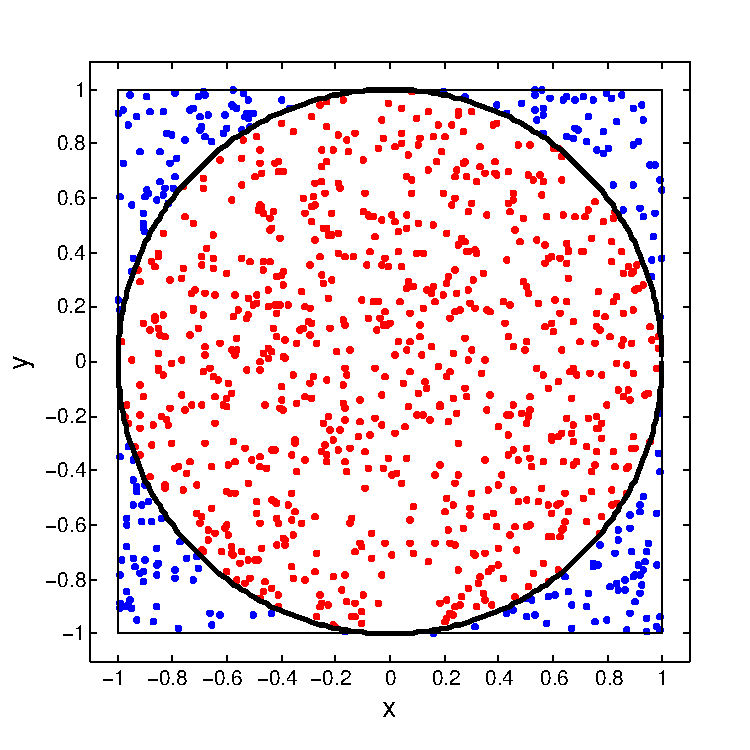
\includegraphics[width=2.0in]{15.Random-Numbers/circle.pdf}
	\caption{Monte Carlo method to evaluate the area inside a circle.  The area inside the circle equals $4 N_\text{red}/(N_\text{blue}+N_\text{red})$ where the factor 4 is the area of the square.}
	\label{fig:MC_circle}
\end{figure}

Multidimensional integrals can be computationally demanding.  There is a way to estimate them by random sampling.  The result may not be very accurate but gives a rough estimate and particularly efficient for high dimensional integral.  Here we evaluate the volume of a $n$-dimensional hypersphere of radius 1.  The sphere is inscribed in a hypercube of edge length 2. The volume of the hypercube is $2^n$.  Now, we generates many random points uniformly distributed in the hypercube. Then, we count the number of points inside the hypersphere.  The ratio of the population inside the sphere and the total population of the points is roughly speaking in proportion to the volume of the sphere to the volume of the cube. Since we know the volume of the cube, we can estimate the volume of the sphere from the ratio. As the number of the points increases to infinity, the result approaches to the exact volume $V_n=\pi^{n/2} / \Gamma(n/2+1)$ where $\Gamma(\cdot)$ is the gamma function.\cite{gamma_function} Figure \ref{fig:MC_circle} illustrates  the case for $n=2$. Generate a pair of standard uniform random numbers $r_1$ and $r_2$.  Convert them to $x$ and $y$ coordinates by 
\begin{equation}
x = 2 r_1 - 1, \qquad y=2 r_2-1
\end{equation}
which are uniform random numbers between $-1$ and $1$.  If $x^2+y^2 < 1$, then increment $N_\textsc{in}$ by one.  After $N$ random points, the volume of the sphere is estimated by $V_\text{sphere} = \frac{N_\textsc{in}}{N} V_\text{cube}$.

Program \ref{prog:vol_sphere} evaluates the volume of the $N$-dimensional hypersphere using the Monte Carlo integration. Figure \ref{fig:MC_hypersphere} shows that with 100000 sampling,
we can evaluate the volume of two-dimensional circle rather accurately and the volume of the six-dimensional sphere within $\pm 5\%$ of error.
If we use a standard integral method, the number of grid points increases as the power of $N$. On the other hand, the number of sampling points necessary to get a reasonable estimate by the Monte Carlo method increases slower than that.  Therefore, the Monte Carlo method is advantageous for high dimensional integrals.

\begin{figure}
\centering
	\begin{subfigure}{0.45\textwidth}
		\centering
		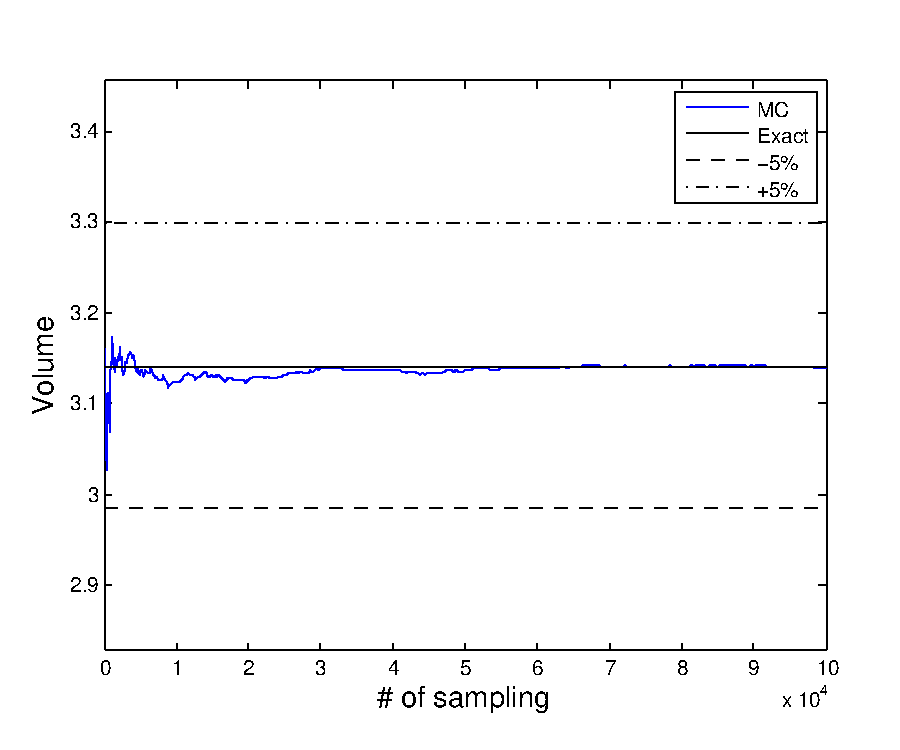
\includegraphics[width=2.5in]{15.Random-Numbers/v2.pdf}
		\caption{2D}
	\end{subfigure}
	\begin{subfigure}{0.45\textwidth}
		\centering
		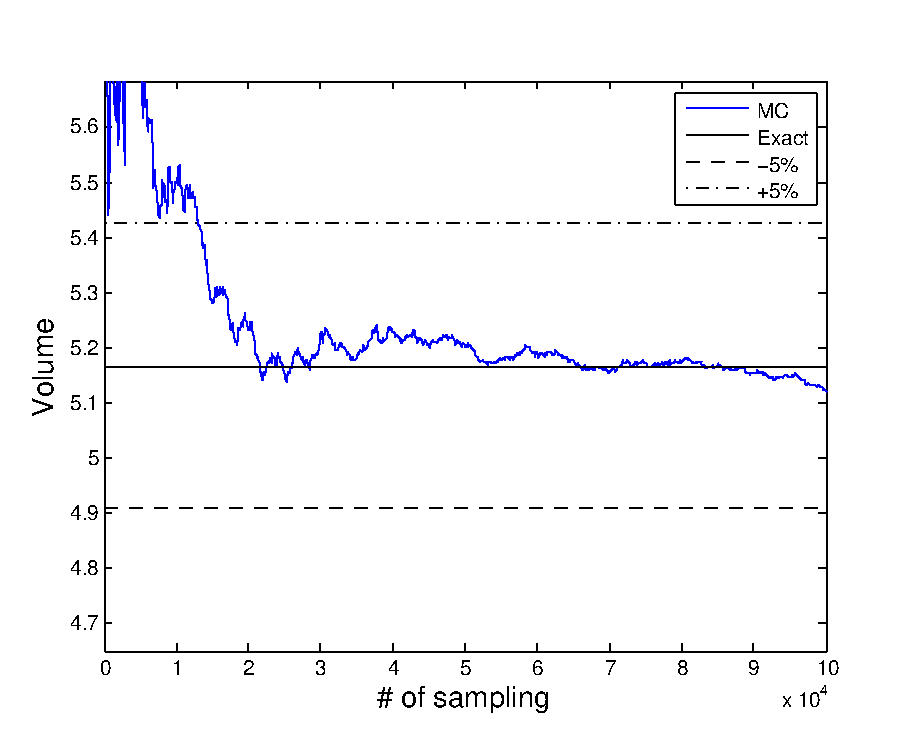
\includegraphics[width=2.5in]{15.Random-Numbers/v6.pdf}
		\caption{6D}
	\end{subfigure}
\caption{Monte Carlo evaluation of the volume of hypersphere. As the number of sampling points increases, the result approaches to the exact value.}
\label{fig:MC_hypersphere}
\end{figure}
\end{example}

\noindent
\section{Non-uniform distributions}

In the previous examples, we generated desired random numbers by stretching space or using two random numbers to cover two-dimensional space.
In either cases, the resulting new random numbers are distributed uniformly.  However, non-uniform distributions are common in physics.  For example, the velocity of the gas particles in thermal equilibrium is Gaussian distributed (Maxwell's distribution).  The chance you find a slow particle is higher than a fast particle.  Since computer systems usually supply only uniform random numbers, we need to transform it to a desired distribution.

Let $\hat{X}$  a stochastic variable and  its realization is a random number $x$ with a distribution $\chi(x)$. We introduce a new stochastic variable $\hat{Y}=f(\hat{X})$.  The realization of $\hat{Y}$ is related to the realization of $\hat{X}$ through the same function $y=f(x)$.
Then, the mathematical theorem tells that
\begin{equation}
\rho(y) |\md y| = \chi(x) |\md x|
\end{equation}
and thus we have the distribution of $y$ as
\begin{equation}\label{eq:1d_transform1}
\rho(y) = \chi(x)\left | \frac{\md x}{\md y} \right | = \chi(x) \left | \frac{ \md f^{-1}(y)}{\md y} \right |.
\end{equation}
If $x$ is uniformly distributed as
\begin{equation}\label{eq:uni_dist}
\chi(x) = \begin{cases} 1 & 0<x<1 \\[1ex]
0 & \text{otherwise} \end{cases}
\end{equation}
then we have
\begin{equation}\label{eq:1d_transform2}
\rho(y) =  \left | \frac{\md x}{\md y} \right | = \left | \frac{ \md f^{-1}(y)}{\md y} \right |
\end{equation}
By choosing an appropriate function $y=f(x)$, we can construct a random number generate with a desired distribution $\rho(y)$.  For example,
when $y=-\ln(x)$, $\rho(y)=\me^{-y}$.  Figure \ref{fig:expmap} shows the mapping from uniform $x$ between 0 and 1 to $y$ exponentially distributed from 0 to $\infty$.


\begin{figure}
\centering
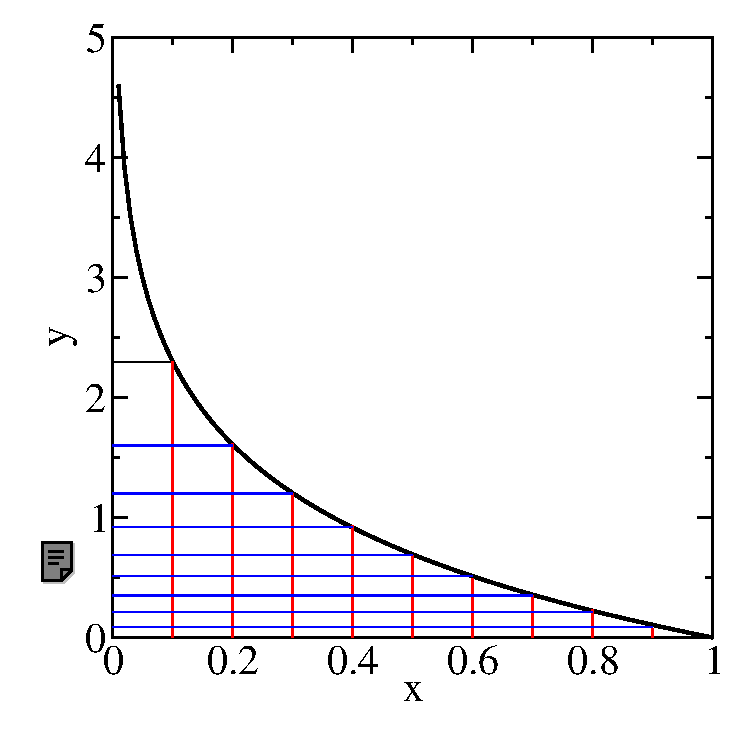
\includegraphics[width=2.5in]{15.Random-Numbers/expmap.pdf}
\caption{Mapping from random number $x$ uniformly distributed between 0 and 1 to $y$ exponentially distributed from 0 to $\infty$.  The transformation function is $y=-\ln(x)$.}
\label{fig:expmap}
\end{figure}


For multi-dimensional cases like Example \ref{ex:n_ball}, we consider a transformation $y_i= f_i(x_1, x_2, \cdots)$.
The distribution for $\{y_i\}$ is given by
\begin{equation}\label{eq:nd_transform}
\rho(y_1, y_2, \cdots) \md y_1 \md y_2 \cdots = \chi(x_1, x_2, \cdots ) \left | \frac{\partial (x_1, x_2, \cdots)}{\partial (y_1, y_2, \cdots)} \right |
\end{equation} 
where $|\partial ()/\partial ()|$ is the Jacobian determinant.  For two-dimensional case, 
\begin{equation}\label{eq:2d_transform}
\rho(y_1, y_2) = \chi(x_1, x_2) \left | \begin{matrix} \frac{\partial x_1}{\partial y_1} & \frac{\partial x_1}{\partial y_2} \\[1.5ex]
 \frac{\partial x_2}{\partial y_1} & \frac{\partial x_2}{\partial y_2} \end{matrix} \right |
\end{equation}

\noindent
\section{Gaussian random number}

Stochastic variables with a Gaussian distribution is defined by 
\begin{equation}\label{eq:Gaussian}
\rho(x) = \frac{\sigma}{\sqrt{2 \pi}} \me^{-x^2/2 \sigma^2}
\end{equation} 
and  it has mean $\mean{x}=0$ and variance $\mean{x^2} - \mean{x}^2=\sigma^2$.  When $\sigma^2=1$, it is called normal distribution.
The Gaussian distributed stochastic variables are ubiquitous particularly in statistical physics. For example, many fluid particles collide with a Brownian particle during a short period of time. The force exerted on the Brownian particle by the fluid particle is stochastic and Gaussian distributed. 

There is a mathematical reason why the normal distribution is ubiquitous. Consider $N$ independent stochastic variables  $X_i,\,  i=1, \cdots, N$ with an identical distribution. The mean and variance are given by $\mean{X_i}=\mu$ and $\mean{(X_i-\mu)^2}=\sigma^2$.  Then, the distribution of a stochastic variable defined by 
\begin{equation}
S_N = \frac{X_1 + X_2 + \cdots + X_N - N \mu}{\sqrt{N \sigma^2}} = \frac{1}{\sqrt{N \sigma^2}} \sum_{i=1}^N (X_i - \mu)
\end{equation}
approaches a normal distribution as $N \rightarrow \infty$.  This is known as central limit theorem.\cite{central_limit_theorem} Note that the distribution of $X_i$ does not have to be Gaussian.  As long as the mean and variance are well defined, the sum of such non-Gaussian stochastic variables is Gaussian distributed.

Now, we want to generate random numbers drawn from the normal distribution.  The normally distributed random generator returns values close to 0 more often than larger values.  One way is to utilize the central limit theorem. Consider 12 random numbers $X_i,\, i=1, \cdots, 12$ uniformly distributed between 0 and 1. As discussed in the previous section, $X_i$ has mean $\mu=1/2$ and variance $\sigma^2=1/12$.  While $N$ is not close to $\infty$, the sum of the 12 random numbers,
\begin{equation}
S_{12} = \frac{X_1 + X_2 + \cdots + X_{12} - 12 \mu}{\sqrt{12 \sigma^2}} = \sum_{i=1}^{12} X_i - 6
\end{equation}
is, roughly speaking, normally distributed.  A main problem of this method is that the largest value it can generate is only 6.  The true normal distribution allows very large number up to infinity although the probability to  obtain such a large value is very small. The probability density at $x=6$ is about $10^{-8}$.  Only one out of 100 million realizations hits that high value.  Hence, it is not a significant deficiency for most applications.  If such rare events are not important, the sum of 12 uniform random numbers is a simple way to generate the normal distribution.  Figure \ref{fig:normal12} shows the distribution of $S_{12}$ which matches well to the true normal distribution.

\begin{figure}
	\centering
	\begin{subfigure}{0.45\textwidth}
		\centering
		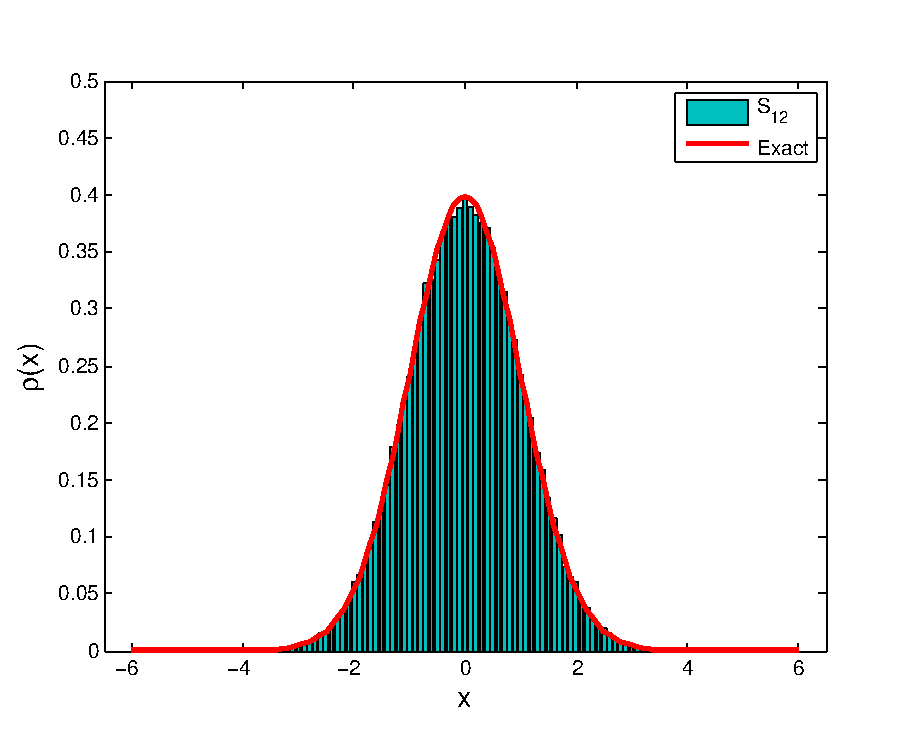
\includegraphics[width=2.5in]{15.Random-Numbers/normal12.pdf}
		\caption{The sum of 12 uniform random numbers}
		\label{fig:normal12}
	\end{subfigure}
	\begin{subfigure}{0.45\textwidth}
		\centering
		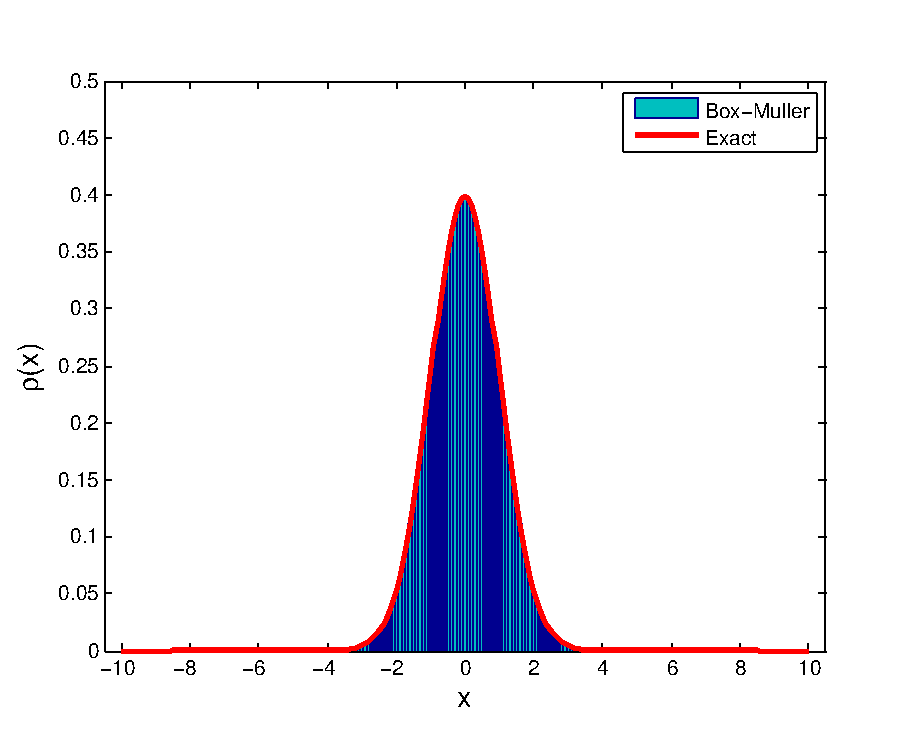
\includegraphics[width=2.5in]{15.Random-Numbers/box-muller.pdf}
		\caption{Box-Muller mnethod}
		\label{fig:box-muller}
	\end{subfigure}
\caption{Two generators of normally distributed random generator.  The distribution is constructed from 100,000 realizations. The distribution of $S_{12}$ is strictly zero for $|x|>6$ and thus rare events are not included. In principle, the Box-Muller method can generate rare random numbers.  However, it is so rare that $|x|>6$ is not realized with this 100,000 sampling.}
\end{figure}

If rare events need to be taken into account, use a mathematically rigorous transformation known as the Box-Muller method.  It turns out that the transformation of two uniformly distributed random numbers $x_1$ and $x_2$ to the two Gaussian distributed random numbers $y_1$ and $y_2$ is more convenient.  Consider the transformations
\begin{subequations}
\begin{eqnarray}
y_1 &=& \sqrt{-2 \ln x_1} \cos(2\pi x_2) \\
y_2 &=& \sqrt{-2 \ln x_1} \sin(2\pi x_2)
\end{eqnarray}
\end{subequations}
and their inverse 
\begin{subequations}
\begin{eqnarray}
x_1 &=& \exp^{-(y_1^2+y_2^2)/2} \\
x_2 &=& \frac{1}{2\pi} \arctan \frac{y_2}{y_1}
\end{eqnarray}
\end{subequations}
The corresponding distribution function for $y_1$ and $y_2$ is
\begin{equation}
\rho(y_1,y_2) =  \left | \begin{matrix} \frac{\partial x_1}{\partial y_1} & \frac{\partial x_1}{\partial y_2} \\[1.5ex]
 \frac{\partial x_2}{\partial y_1} & \frac{\partial x_2}{\partial y_2} \end{matrix} \right |
 = - \left ( \frac{1}{\sqrt{2\pi}} \me^{-y_1^2/2} \right ) \left ( \frac{1}{\sqrt{2\pi}} \me^{-y_2^2/2} \right )
\end{equation}
This distribution indicates that $y_1$ and $y_2$ are independent and normally distributed random numbers. Using two uniformly distributed random numbers $x_1$ and $x_2$, we generate two normally distributed random numbers.  Unlike, the sum of 12 random numbers, $y_1$ and $y_2$ are truly Gaussian distributed from $-\infty$ to $\infty$. 


\begin{example}

\begin{figure}
\centering
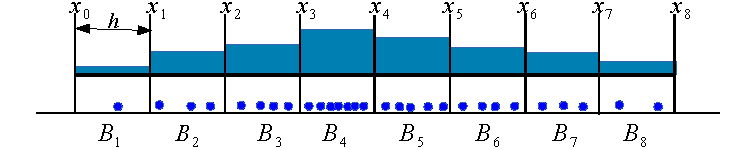
\includegraphics[width=4in]{15.Random-Numbers/histogram.pdf}
\caption{Generating histogram from continuous random numbers.  Circles indicate the random numbers.  The number of the circles in a bin corresponds to the height of the bar above it.}\label{fig:histogram}
\end{figure}

Generate random numbers that are normally distributed.  Program \ref{prog:box-muller} implements the Box-Mullar method.
We check the distribution of random numbers by plotting a histogram. 
To construct a histogram, first we create bins by dividing the entire range into many small intervals.  For eaxmple, one bin corresponds to a segment between $x$ and $x+h$ where $h$ is the width of the bin.  See Fig. \ref{fig:histogram}. 
Now, we generate a random number and check which bin the random number belongs to.  After generating sufficient number of random numbers, count the number of random numbers in each bin.  That is the height of the bar in the histogram.
  Figure \ref{fig:box-muller} shows the distribution of random numbers generated by  the Box-Muller method. The width of the bins is
   very small in this plot and the plot looks like continuous line,  However. it is a histogram.
\end{example}


\noindent
\subsection{Exponential distributions}

An exponential distribution with a rate parameter $\lambda>0$ defined by
\begin{equation}\label{eq:exp_dist}
\rho(x) = \begin{cases} \lambda \me^{-\lambda x} & x > 0 \\[1ex]
0 & x < 0 \end{cases}
\end{equation}
and its mean and variance are $\mu=1/\lambda$ and $\sigma^2=1/\lambda^2$.

The exponential distribution is also common in physics. For example, the energy of a system in a thermal equilibrium is a stochastic variable and distributed exponentially as
\begin{equation}
\rho(E) = \frac{1}{Z} \me^{-E/\kB T}
\end{equation}
where $Z$ is a normalization constant. This distribution is known as the  Boltzmann distribution. 

The exponentially distributed random numbers can be obtained by a transformation $y=-\ln(x)/\lambda$ where $x$ is a uniformly distributed between 0 and 1.

\noindent
\subsection{Evaluation of Mean}

To analyze stochastic systems, we often evaluate a mean of a physical quantity $f(\hat{X})$ which is a function of stochastic variable $\hat{X}$.  The analytic expression is defined by 
\begin{equation}
\mean{f} = \sum_i f(x_i) P_i
\end{equation}
for a discrete system
and 
\begin{equation}
\mean{f} = \int f(x) \rho(x) \md x
\end{equation}
for a continuous system.
We evaluate this summation or integral using the Monte Carlo method.  The procedure is very simple.
Generate $N$ random numbers $r_i,\, i=1,\cdots,N$ out of a desired distribution $P_i$ or $\rho(x)$.  The mean is simply
\begin{equation}
\mean{f} = \lim_{N \rightarrow \infty} \frac{1}{N} \sum_{i=1}^N f(r_i) 
\end{equation}
Of course, in practice, we use a finite number of sampling $N$.  We need to make it sure that $N$ is large enough to get an accurate value.

\begin{example}

Consider a stochastic variable $\hat{X}$ of normal distribution. We evaluate the 2nd and 4th moments, $\mean{x^2}$ and $\mean{x^4}$, using the Monte Carlo method. It is known that $\mean{x^4} = 3 \mean{x^2}^2$. We will check if the Monte Carlo simulation can get the same answer. Program \ref{prog:normal_dist} evaluates the moments using the Box-Muller method.   With $N=1000$, the agreement is not bad but 
much better agreement is obtained with $N=1000000$.

\begin{center}
\begin{minipage}{3.5in}
\small
\begin{Verbatim}[frame=single]
N=   1000000,  V4/(V2)^2 = 3.0009e+00
N=      1000,  V4/(V2)^2 = 2.9033e+00
\end{Verbatim}
\normalsize
\end{minipage}
\end{center}
\end{example}


\noindent
\section{Applications in Physics}

\subsection{Thermal Speed}

Particles in a three-dimensional gas at temperature $T$ has random velocity $v$ and its probability distribution of the velocity is given by the Maxwell's distribution
\begin{equation}
\rho(\vb{v}) = \sqrt{\frac{m}{2 \pi \kB T}} \me^{-m v^2/2 \kB T}
\end{equation}
where $m$ is the mass of the particle and $T$ and $\kB$ are temperature of the gas and the Boltzmann constant, respectively.
The mean velocity is clearly $\mean{v}=0$ since $v$ and $-v$ have the equal probability.  On the other hand, the mean \emph{speed} does not vanish. The exact answer can obtained as
\begin{equation}\label{eq:mean_speed}
\mean{|v|} = \iiint |v| \rho(\vb{v}) \dd{v_x} \dd{v_y} \dd{v_z} =\sqrt{\frac{m}{2 \pi \kB T}}\int_0^\infty \int_0^\pi \int_0^{2\pi} v^3 \me^{-m v^2/2 \kB T} \dd{\phi} \sin\theta \dd{\theta} \dd{v} = \sqrt{\frac{8 \kB T}{\pi m}}
\end{equation}

Now, we try to evaluate the mean \emph{speed} of hydrogen molecules in the air  using the random numbers.  Since the Maxwell's distribution is Gaussian, we can use the normally distributed random numbers with mean value $\mu=0$ and variance $\sigma=\sqrt{\frac{\kB T}{m}}$. Here, as an exercise, we try to confirm Eq. \eqref{eq:mean_speed}  by the direct Monte Carlo simulation. 

The statistical analysis tells that the relative error of the finite sampling is about $1/\sqrt{N}$.
Therefore, with $N=100000$ sampling, we expect $\frac{\Delta v}{\mean{|v|}} \sim 10^{-4}$.  Program \ref{prog:mean_ke} generates
normally distributed random numbers $\vb{v}_i$ and calculates the mean speed $\mean{|v|} = \frac{1}{N} \sum_i^{N} |v_i|$.  The result shows the error less than $10^{-4}$ as expected.

\begin{center}
\begin{minipage}{4in}
\small
\begin{Verbatim}[frame=single]
mean speed = 1.77558e+03 (exact=1.77566e+03)
relative error = 4.6397e-05
\end{Verbatim}
\normalsize
\end{minipage}
\end{center}

\noindent
\subsection{Sedimentation-diffusion equilibrium}

A colloidal particle of mass $m$ under the uniform gravity $g$ does not fall down completely to the bottom of the container.  Random collisions with the fluid particles push the colloidal particle upward against the gravity. The height of the particle from the bottom is stochastic and distributed as
\begin{equation}\label{eq:barometric}
\rho(z) = \frac{m g}{\kB T} \me^{- m g z/\kB T}
\end{equation}
which is known as barometric formula.\cite{barometric}  The barometric formula is one of the example of the Boltzmann distribution.
Two hundred colloidal particles are placed in a fluid.  Generate an image showing the location of the colloidal particles.

Measure the height using  the gravitational length $\ell_g = \kB T/m g$ as unit, the distribution is simply
\begin{equation}
\rho(z) = \me^{-z}
\end{equation}
The horizontal positions of the particles are uniformly distributed whereas the vertical positions are exponential.  Program \ref{prog:sediment} generates a snapshot image of the sedimentation-diffusion equilibrium.  The result is shown in Fig. \ref{fig:sediment}.  The distribution of particles obtained by the Monte Carlo simulation resembles to the experimental observation.

\begin{figure}
	\centering
	\begin{subfigure}{0.45\textwidth}
		\centering
		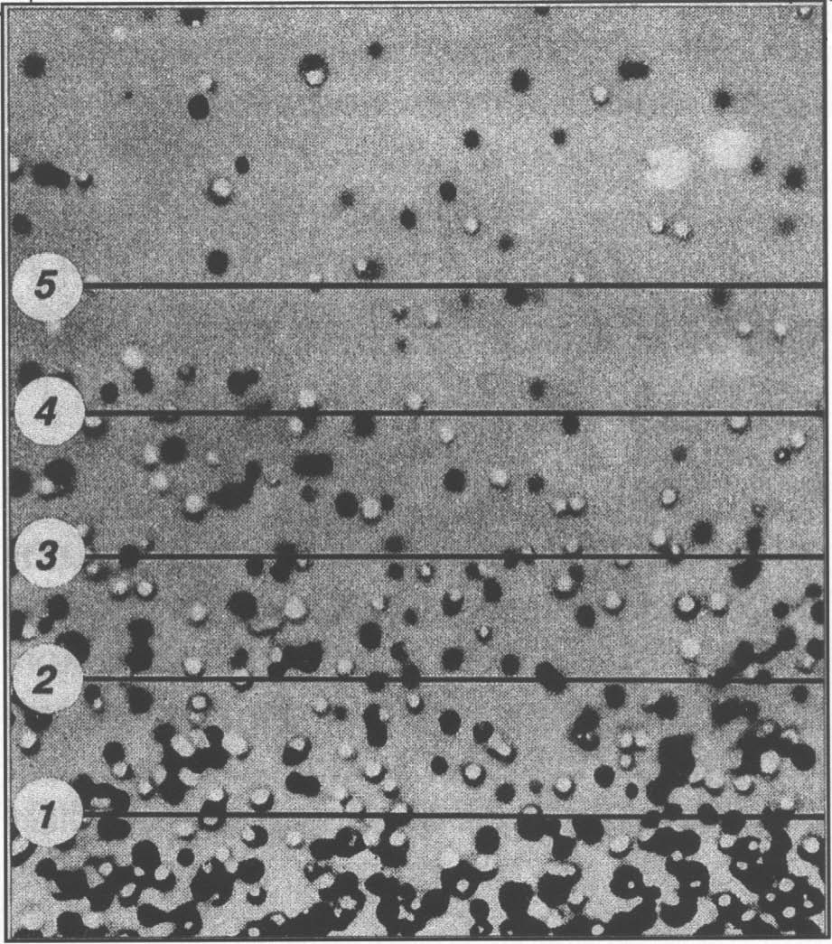
\includegraphics[width=1.8in]{15.Random-Numbers/sediment.pdf}		
		\caption{Experiment}
	\end{subfigure}
	\begin{subfigure}{0.45\textwidth}
		\centering
		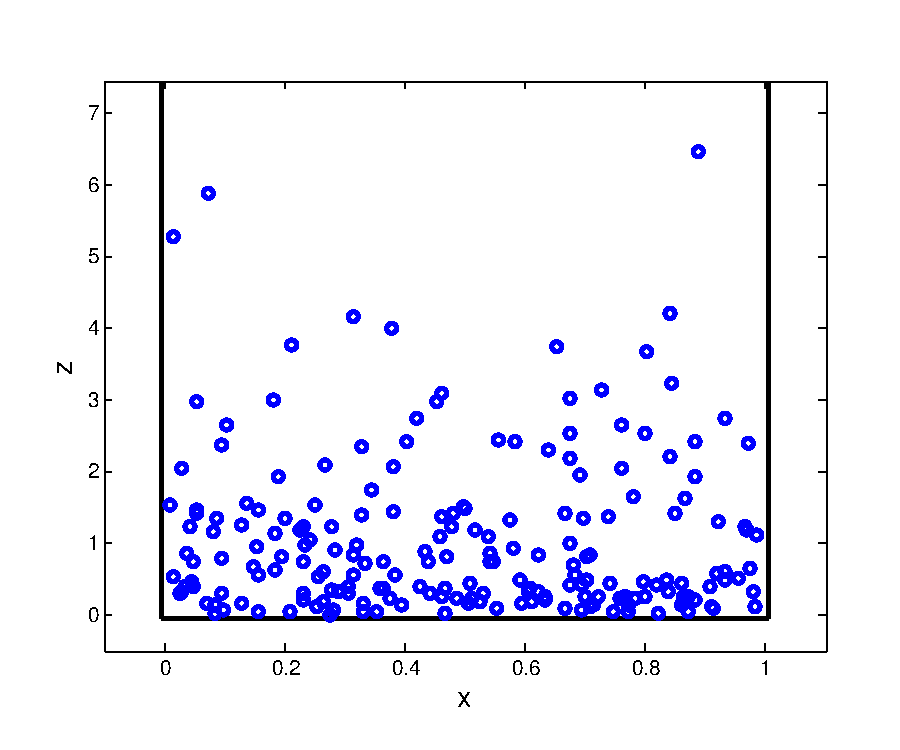
\includegraphics[width=2.5in]{15.Random-Numbers/sediment2.pdf}
		\caption{Exponential Distribution}
	\end{subfigure}
	\caption{Snapshot of the sedimentation diffusion equilibrium}\label{fig:sediment}
\end{figure}

\noindent
\subsection{Surface Growth: Random Deposition Models}

\begin{figure}
	\centering
	\begin{subfigure}{0.45\textwidth}
		\centering
		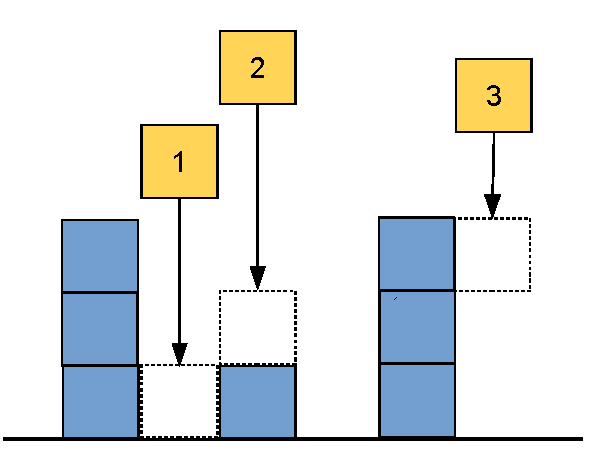
\includegraphics[width=2.0in]{15.Random-Numbers/deposition_model1.pdf}
		\caption{Ballistic deposition model with or without overhang.}
		\label{fig:ballistic_deposition1}
	\end{subfigure}
	\begin{subfigure}{0.45\textwidth}
		\centering
		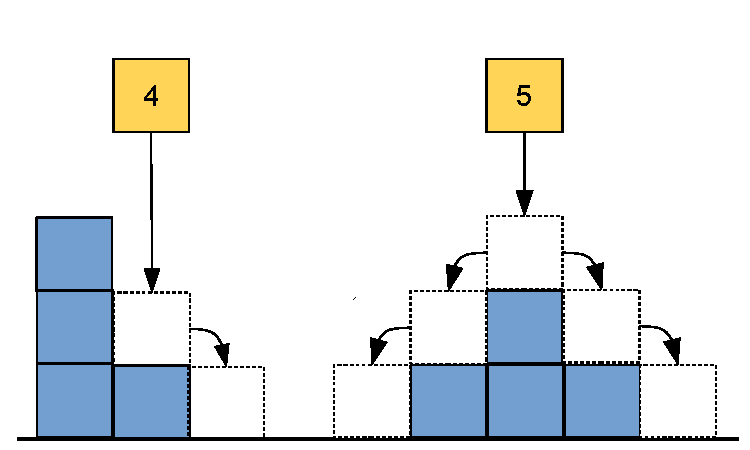
\includegraphics[width=2.5in]{15.Random-Numbers/deposition_model2.pdf}
		\caption{Ballistic deposition model with surface relaxation.}
		\label{fig:ballistic_deposition2}
	\end{subfigure}
	\caption{A random deposition model with surface relaxation.  The lateral position is randomly selected and a particle is placed on the surface particle from the above.  Then, it steps down to the local minimum.} 
	\label{fig:deposition_model}
\end{figure}


The current technology demands high quality of materials. Crystals grows by themselves but we want to control the growth of the materials.  The vapor deposition method and molecular beam epitaxy (MBE) allow us to deposit atoms on top of the substrate in a controlled manner.  We want to simulate such a surface growth process in computer.  A simplest model is the random deposition model.\cite{ballistic_growth} (See Fig. \ref{fig:ballistic_deposition1}.)
The lateral position of the particles are randomly chosen.  Particles either falls down to the substrate (particle 1 in Fig \ref{fig:ballistic_deposition1}) or stick to on top of the other particle (particle 2).  It is interesting that even we choose the lateral position of the particles by uniform random numbers, the resulting surface is not smooth at all. This model generates a densely packed crystal but with large surface roughness.  

In order to quantify the surface roughness, we first define the height of the surface as a stochastic variable. We consider a one-dimensional substrate of the size $L$ and deposit $N$ particles on it.  As particles are deposited, the surface grows.  However, the growth is not uniform. The height $h_i$ at the lateral position $x_n,\, n=1,\cdots, L$ is random number drawn out of a certain probability distribution $P(h;N)$, which we want to find by computer simulation. 
We calculate the mean height and the second moment by
\begin{equation}
\mean{h} = \frac{1}{L} \sum_{i=1}^L h_i, \qquad \mean{h^2} = \frac{1}{L} \sum_{i=1}^L h_i^2,
\end{equation}
Rigorously speaking $L$ should be infinitely large but in computer we use a large finite number.  In order to get a good statistics, we need a large surface area.  Alternatively, we can simulate many copies of a smaller surface and add them up for statistical calculation. 

Now, we define the surface roughness as variance of the height
\begin{equation}
w = \sqrt{\mean{h^2}-\mean{h}^2}.
\end{equation}
For the simple random deposition model, we can calculate it analytically.  The probability that the particle hits a lateral position is $p=1/L$.  The probability distribution of the height $h$ after $N$ particles are deposited is given by a binomial distribution
\begin{equation}
P(h;N) = \frac{N!}{h! (N-h)!} p^h (1-p)^{N-h}\quad \xrightarrow[N \rightarrow \infty]{}\quad \frac{1}{\sqrt{2\pi w^2}} \me^{-(h-\mean{h})^2/2 w^2}.
\end{equation}
The mean height is 
\begin{equation}
\mean{h} = \sum_{h=1}^{N} h P(h;N) = N p = \frac{N}{L}
\end{equation}
which grows linearly with $N$ as expected.  The surface roughness is 
\begin{equation}\label{eq:roughness_evolution}
w = \sqrt{N p (1-p)} = \sqrt{\frac{N}{L}(1-1/L)} \approx \sqrt{\frac{N}{L}} = \sqrt{\mean{h}}.
\end{equation}
As the height of the surface grows, the roughness also grows but as the sqrt of the height.

\begin{figure}
	\centering
	\begin{subfigure}{0.45\textwidth}
		\centering
		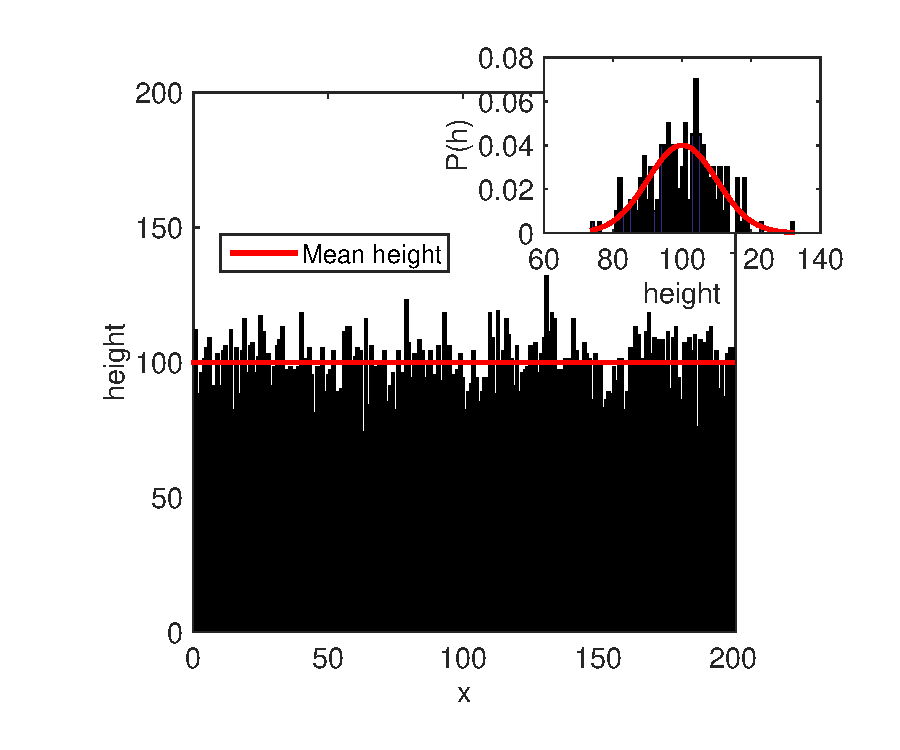
\includegraphics[width=2.9in]{15.Random-Numbers/bd1-height.pdf}	
		\caption{Surface roughening.  (Inset: Height distribution)}
		\label{fig:bd1_height}
	\end{subfigure}
	\begin{subfigure}{0.45\textwidth}
		\centering
		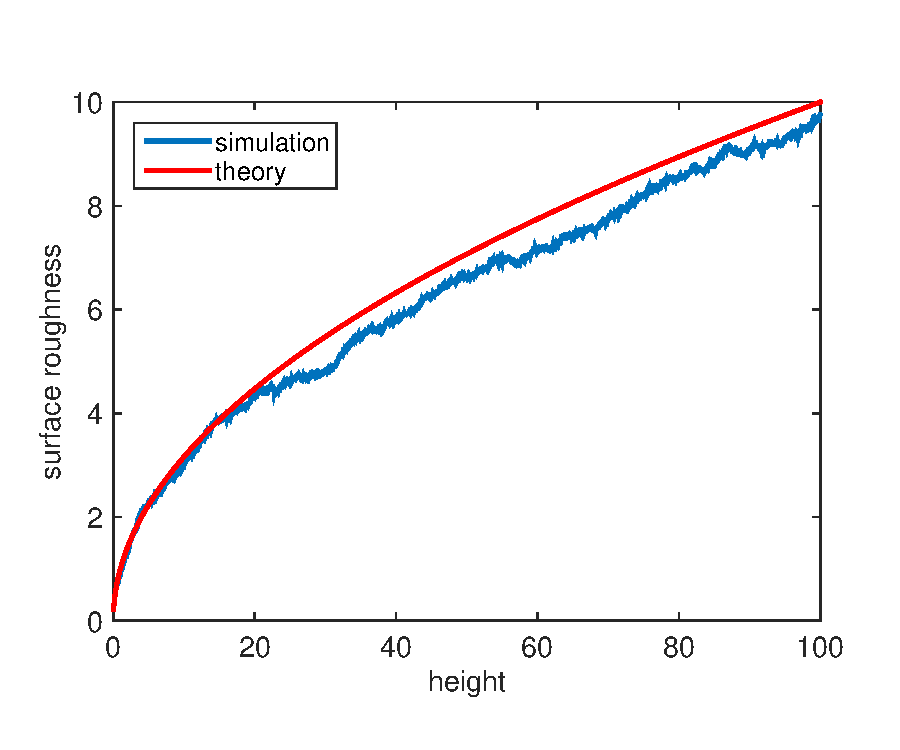
\includegraphics[width=2.5in]{15.Random-Numbers/bd1-roughness.pdf}
		\caption{Growth of surface roughness.}
		\raisebox{6pt}{}
		\label{fig:bd1_roughness}
	\end{subfigure}
	\caption{Surface growth with the ballistic deposition model without surface relaxation.}\label{fig:bd1}
\end{figure}

Now we turn to the simulation.  Here is the algorithm.
\bigskip
\begin{myalgobox}
\Algorithm{Ballistic deposition model without surface relaxation}

\medskip
\begin{minipage}{5.5in}
\begin{enumerate}
\item Set the height of the surface $y(x)$ to zero at all position $x=, \cdots, L$.
\item Generate a random position $x$ between $1$ and $L$. 
\item Deposit the particle at $x$.  (Increment $y(x)$ by one.
\item Repeat the deposition for $N$ times.
\item Evaluate the mean height and the roughness.
\end{enumerate}
\end{minipage}

\end{myalgobox}


\bigskip
Program \ref{prog:bd1} impliments this algorithm.
Figures \ref{fig:bd1} show the results.  The suraface size $L=200$ and the number of particles $N=100,000$ are used. 
The profile of the surface (Fig. \ref{fig:bd1_height}) shows that the surface is not smooth at all.  Some part is much higher and other part much lower than the average height.  The inset plots the distribution of height. The different between the higest and the lowest height is as big as 50, a half of the mean height!  Figure \ref{fig:bd1_roughness} plots the growth of the surface roughness as a function of the mean height.  The result of the simulation agrees with the theory (\ref{eq:roughness_evolution}).  The simulation data is noisy because the surface area $L=200$ is not big enough to get a good statistics.

The above result is a bit unrealistic since the surface roughness is not so big in the real matrials.
A problem of the simple random deposition model is the surface roughness increases indefinitely, which  never happens in the real world.  A reasonable modification to the simple random deposition is to include the effect of the surface diffusion.\cite{surface_relaxation}  Once a particle is absorbed on to the surface, it can diffuse on the surface until it find a more stable position.  It is called surface relaxation.  It can be model by a biased random walk.  The particle moves to a neighbor site lower than the present site. (See particle 4 in Fig. \ref{fig:ballistic_deposition2}.)  If there are multiple sites lower than the present site, one of them are picked at random. (See particle 5 in Fig. \ref{fig:ballistic_deposition2}.)
When the surface relaxation is taken into account, the roughness grows as $w = \mean{h}^\beta$ up to a certain value where $\beta$ is called the growth exponent.  When the mean height reaches a crossover height $h_c$, the roughness does not grow any loner and stay the same.\cite{surface_relaxation}

The following algorithm adds the surface relaxation to the ballistic deposition model.

\bigskip

\begin{myalgobox}
\Algorithm{Ballistic deposition model with surface relaxation}

\medskip
\begin{minipage}{5.5in}
\begin{enumerate}
\item Set the height of the surface $y(x)$ to zero at all position $x=, \cdots, L$.
\item Generate a random position $x$ between $1$ and $L$. 
\item If $y(x-1) \geq y(x)$ and $y(x+1) \geq y(x)$, then deposit it at $x$. Go to Step 7.
\item If $y(x-1) < y(x)$ and $y(x+1) > y(x)$, then 
\begin{itemize}
\item If $r<0.5$, then $x=x-1$ (jump to the left).  
\item Otherwise, $x=x+1$ (jump to the right).
\item Go back to Step 3.
\end{itemize}
\item $if y(x-1)> y(x)$, then $x=x+1$ (jump to the right).  Go back to Step 3.
\item The last possibility is $y(x+1)>y(x)$.  Thus, $x=x-1$ (jump to the left).  Go back to Step 3.
\item Repeat the deposition for $N$ times.
\item Evaluate the mean height and the roughness.
\end{enumerate}
\end{minipage}

\end{myalgobox}


\begin{figure}
	\centering
	\begin{subfigure}{0.45\textwidth}
		\centering
		\raisebox{12pt}{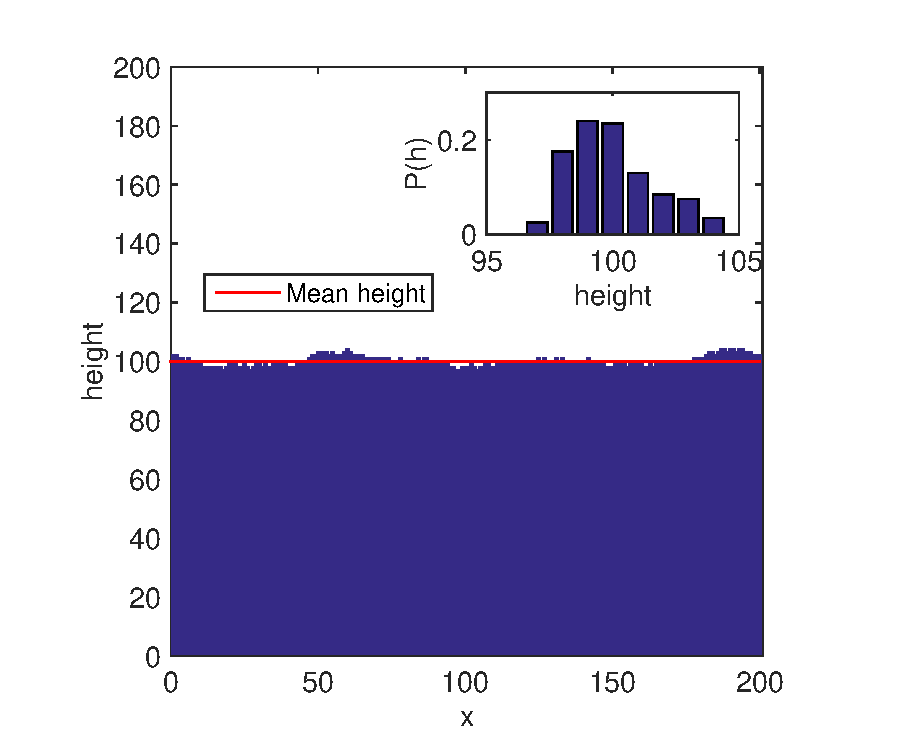
\includegraphics[width=2.5in]{15.Random-Numbers/bd2-height.pdf}}	
		\caption{Surface roughening.}
		\label{fig:bd2_height}
	\end{subfigure}
	\begin{subfigure}{0.45\textwidth}
		\centering
		\raisebox{6pt}{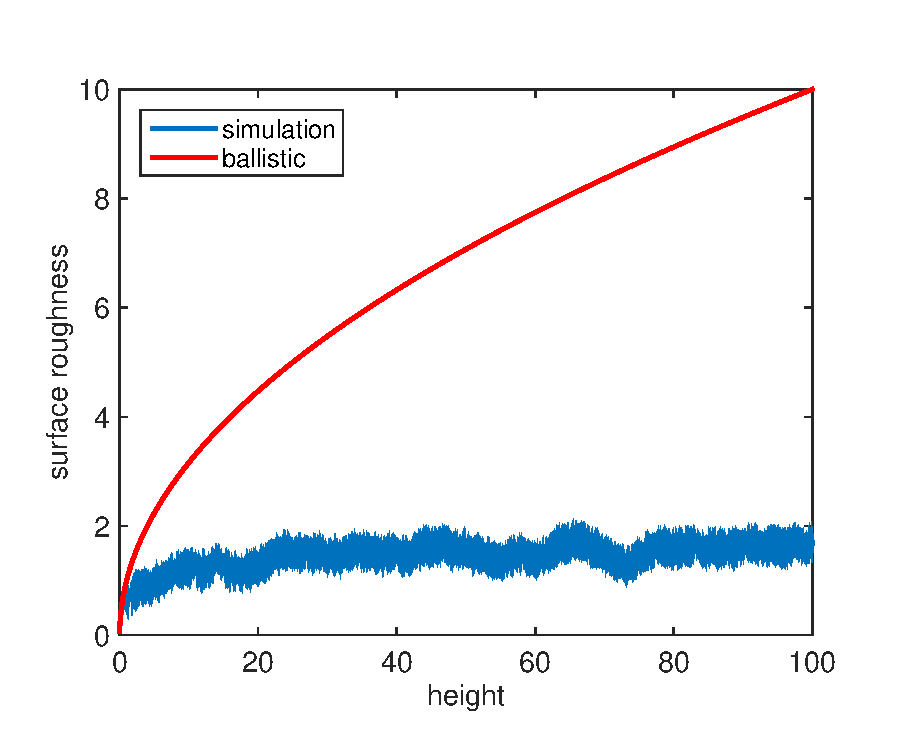
\includegraphics[width=2.5in]{15.Random-Numbers/bd2-roughness.pdf}}
		\caption{Growth of surface roughness.}
	\end{subfigure}
	\caption{Surface growth with the ballistic deposition model with surface relaxation.}\label{fig:bd2}
\end{figure}

Program \ref{prog:bd2} impliments the algorithm and simulate the surface growth with relaxation.   The results are plotted in Figures \ref{fig:bd2}.  The surface profile plotted in \ref{fig:bd2_height} indicates the the surface is much smoother now. The height distribution in the inset shows that the difference between the highest and lowest is less than 10.  The growth of the surface roughness shown in Fig. \ref{fig:bd2_roughness} suggests that the roughness deos not grow after initial growth.  Threfor,e this model is more realistic than the simple ballistic deposition model.

Finally, we includes a possibility to form the overhang (particle 3 in Fig. \ref{fig:ballistic_deposition1}) in Program \ref{prog:bd3}.  
No surface relaxation is considered.  Theresulting materials is highly porous. The profile of the surface plotted in Fig. \ref{fig:bd3_height} shows many hollow regions. After $N=200,000$ particles is deposited, the surface height reached nearly $200$ which is twice as high as the previous growth models, indicating that almost a half of the space is not filled.  Note also that  the size of the empty space varies widely.  See Ref. \cite{ballistic_growth} for the detailed discussion of this growth pattern, 

\begin{figure}
\centering
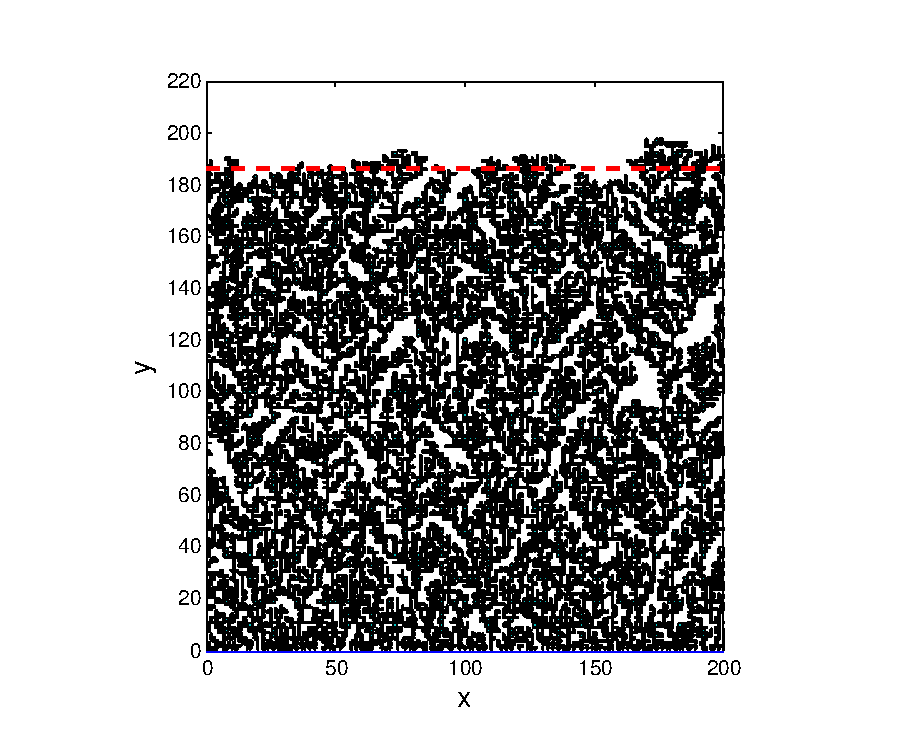
\includegraphics[width=3in]{15.Random-Numbers/bd3-height.pdf}
\caption{Growth of a surface based on a ballistic deposition model with possibility of overhang structures.}
\label{fig:bd3_height}
\end{figure}

\noindent
\section{Problems}

\begin{enumerate}[labelwidth=0.5cm,labelindent=0cm,leftmargin=*,label=\bfseries \thechapter.\arabic*,align=left]
\item
Using the random numbers, calculate the mean $\mu$ and variance $\sigma^2$ of random numbers uniformly distributed between 0 and 1.  Compare results with the theoretical values.
\item
Find $\mean{|x|}_\text{normal}$ by stochastic calculation and compare the result with the analytic solution.
\end{enumerate}

\newpage
\noindent
\section*{MATLAB Source Codes}
\addcontentsline{toc}{section}{\protect\numberline{}MATLAB Source Codes}


\noindent
\program
\label{prog:virtual_die}
\footnotesize
\begin{lstlisting}[language=matlab]
%**************************************************************************
%*     Example 15.1                                                       *
%*     filename: ch15pr01.m                                               *
%*     program listing number: 15.1                                       *
%*                                                                        *
%*     This program simulate a dice using a psueo random number           *
%*     generator.    (random() in MATLAB is not used.)                    *
%*                                                                        *
%*     Programed by Ryoichi Kawai for Computational Physics Course.       *
%*     Last modification:  02/15/2015.                                    *
%**************************************************************************
clear all

% parapmeters for random number generators
a = int64(16807);
b = int64(0); 
c = int64(2147483647);

% get a seed
x=int64(input('Seed='));

% generate uniform random numbers
N=6000;
for i=1:N
    x = mod(a*x,c);
    r(i)=double(x)/double(c);
end
 
% statistics of virtual die
P(1:6)=0;
for i=1:N
    n=ceil(6*r(i));
    P(n)=P(n)+1;
end

p=bar(P);
set(p,'facecolor',[0,0.75,0.75])
hold on
q=plot([0,7],[1000,1000],'--');
set(q,'color','red')
xlabel('face of die','fontsize',14)
ylabel('number of realization','fontsize',14)
hold off
\end{lstlisting}
\normalsize


\bigskip
\noindent
\program
\label{prog:vol_sphere}
\footnotesize
\begin{lstlisting}[language=matlab]
%**************************************************************************
%*     Example 15.2                                                       *
%*     filename: ch15pr02.m                                               *
%*     program listing number: 15.2                                       *
%*                                                                        *
%*     This program  evaluate the value of pi using the Monte Carlo       *
%*     integeration of a circle.                                          *
%*     Uses: rand() in MATLAB                                             *
%*                                                                        *
%*     Programed by Ryoichi Kawai for Computational Physics Course.       *
%*     Last modification:  02/25/2017.                                    *
%**************************************************************************
clear all
clc

% random points on a square
N=100000;
x=random('unif',-1.0,1.0,[1,N]);
y=random('unif',-1.0,1.0,[1,N]);

% points inside the circle
hit=0;
i=0;
for n=1:N
    if x(n)^2+y(n)^2 < 1
        hit=hit+1;
    end
    if mod(n,100)==0 % evaluate at every 100 
        i=i+1;
        PI(i)=hit/n*4; % estimate of pi
    end
end

p=plot([1:i]*100,PI);
hold on
q=plot([0, N], [pi,pi]);
set(q,'color','black')
xlabel('# of sampling','fontsize',14)
ylabel('V_2','fontsize',14)
axis([0 N pi*0.9 pi*1.1])
hold off
\end{lstlisting}
\normalsize


\bigskip
\noindent
\program
\label{prog:box-muller}
\footnotesize
\begin{lstlisting}[language=matlab]
%**************************************************************************
%*     Example 15.3                                                       *
%*     filename: ch15pr03.m                                               *
%*     program listing number: 15.3                                       *
%*                                                                        *
%*     This program generates Gaussian distributed random numbers         *
%*     using the Box-Muller method.                                       *
%*                                                                        *
%*     Programed by Ryoichi Kawai for Computational Physics Course.       *
%*     Last modification:  02/25/2017.                                    *
%**************************************************************************
clear all

N=10000000;
x = rand(N,2);
y(:,1) = sqrt(-2*log(x(:,1))).*cos(2*pi*x(:,2));
y(:,2) = sqrt(-2*log(x(:,1))).*sin(2*pi*x(:,2));
ymin=min(y(:));
ymax=max(y(:));
fprintf('the largest deviation=%f, %f\n',ymin,ymax)

h=histogram(y,201,'Normalization','pdf');
hold on
% true normal distribution
K=201;
xmin=floor(ymin);
xmax=ceil(ymax);
X=linspace(xmin,xmax,K);
F=exp(-X.^2/2)/sqrt(2*pi);
p=plot(X,F);
set(p,'color','red','linewidth',2)
xlabel('x','fontsize',14)
ylabel('\rho(x)','fontsize',14)
legend('Box-Muller','Exact')
axis([xmin xmax 0.0 0.5])
hold off
\end{lstlisting}
\normalsize


\bigskip
\noindent
\program
\label{prog:normal_dist}
\footnotesize
\begin{lstlisting}[language=matlab]
%**************************************************************************
%*     Example 15.4                                                       *
%*     filename: ch15pr04.m                                               *
%*     program listing number: 15.4                                       *
%*                                                                        *
%*     This program evaluates 1st through 4th moments of normal           *
%*     distribution.                                                      *
%*                                                                        *
%*     Programed by Ryoichi Kawai for Computational Physics Course.       *
%*     Last modification:  02/25/2017.                                    *
%**************************************************************************
clear all;

N=100000;

v=normrnd(0.0,1.0,[N,1]);

fprintf('order    moment\n')
for i=1:4
    m(i)=sum(v.^i)/N;
    fprintf('%3d     % 10.4e\n',i,m(i));
end
r=m(4)/m(2)^2;
fprintf('\nm4/(m2)^2 = %8.4d (exact=3)\n',r)
\end{lstlisting}
\normalsize


\bigskip
\noindent
\program
\label{prog:mean_ke}
\footnotesize
\begin{lstlisting}[language=matlab]
%**************************************************************************
%*     Section 15.5.1                                                     *
%*     filename: ch15pr05.m                                               *
%*     program listing number: 15.5                                       *
%*                                                                        *
%*     This program evaluate the mean speed of the gas particles          *
%*     in a thermal equilibrium.                                          *
%*                                                                        *
%*     Programed by Ryoichi Kawai for Computational Physics Course.       *
%*     Last modification:  02/25/2017.                                    *
%**************************************************************************
clear all;

% parameters
T=300.;  % Temperature in K
k=1.380658e-23; % Boltzman constant in J/K
m=2*1.672623e-27; % H2 mass in kg

% Maxwell distribution
N=1000000;
s=sqrt(k*T/m);
v=normrnd(0.0,s,[N,3]); % 3 components (vx, vy, vz)

% speed
speed=sqrt(v(:,1).^2+v(:,2).^2+v(:,3).^2);
% mean
mean=sum(speed)/N;
% theory
exact=2*s*sqrt(2/pi);
%error
error=abs(mean-exact)/exact;

fprintf('mean speed = %10.5e (exact=%10.5e)\n',mean,exact)
fprintf('relative error = %10.5e\n',error)
\end{lstlisting}
\normalsize


\bigskip
\noindent
\program
\label{prog:sediment}
\footnotesize
\begin{lstlisting}[language=matlab]
%**************************************************************************
%*     Section 15.5.2                                                     *
%*     filename: ch15pr06.m                                               *
%*     program listing number: 15.6                                       *
%*                                                                        *
%*     This program generates distribution of particles under gravity     *
%*     thermal diffusion.                                                 *
%*                                                                        *
%*     Programed by Ryoichi Kawai for Computational Physics Course.       *
%*     Last modification:  02/26/2017.                                    *
%**************************************************************************
clear all

N=1000; % number of particles

x=rand(N,1); %horizontal position = uniform
y=rand(N,1); % vertical position = exponential
z=-log(y);
zmax=max(z(:))+1;

subplot(1,2,1)
p=plot([-0.005 1.005],[-0.05,-0.05], [-0.005,-0.005],...
       [-0.05,zmax],[1.005,1.005],[-0.05,zmax]);
set(p,'color','black','linewidth',2)
hold on
p=plot(x,z,'.');
set(p,'linewidth',2)
axis([-0.1 +1.1 -0.5 zmax])
xlabel('x','fontsize',14)
ylabel('z','fontsize',14)
hold off

subplot(1,2,2)
h=histogram(z,int32(2*zmax),'Normalization','pdf');
hold on
Z=linspace(0.0,zmax,201);
P=exp(-Z);
q=plot(Z,P,'--');
set(q,'linewidth',2,'color','red')
xlabel('z','fontsize',14)
ylabel('probability density','fontsize',14)
hold off
\end{lstlisting}
\normalsize


\bigskip
\noindent
\program
\label{prog:bd1}
\footnotesize
\begin{lstlisting}[language=matlab]
%**************************************************************************
%*     Section 15.5.3                                                     *
%*     filename: ch15pr07.m                                               *
%*     program listing number: 15.7                                       *
%*                                                                        *
%*     This program simulatesa the surface growth using ballistic         *
%*     deposit model.                                                     *
%*                                                                        *
%*     Programed by Ryoichi Kawai for Computational Physics Course.       *
%*     Last modification:  02/26/2017.                                    *
%**************************************************************************
clear all  % clear all variables
close all  % close alll figures

N=20000; % number of particles to be deposited
L=200; % surface area

y=zeros(L,1); % reset the height of the surface
x=ceil(rand(N,1)*L);  % horizontal position of the particles

k=0;
for i=1:N
    y(x(i))=y(x(i))+1;  % ballistic growth
    
    % record the evolution of the growth after every 10 particles is
    % deposited
    if mod(i,10)==0
        k=k+1;
        z(k)=sum(y,1)/L;  % mean height
        w(k)=sqrt(sum((y-z(k)).^2)/L);  % roughness
    end
end

% calculate the height distribution
n1=min(y);  % lowest
n2=max(y);  % heighest
h=zeros(n2-n1+1,1);
for i=1:L
    n=y(i)-n1+1;
    h(n)=h(n)+1;
end
h=h/sum(h);

% theoretical height distribution (Gaussian formula)
mu=real(N)/L;
sg=real(N)*(L-1)/L^2;
g=zeros(n2-n1+1,1);
for n=n1:n2
    g(n-n1+1) = exp(-(n-mu)^2/(2*sg))/sqrt(2*pi*sg);
end

% Figure 1: profile of the surface
b=bar([1:L],y);
hold on
plot([0,L],[0,0]);  % draw the base line
axis equal % fix the aspect ratio (needed for movie)
axis([0 L+1 0 N/L*2])  % fix the axis range
hold on
p=plot([0,L],[z(k),z(k)]);
set(p,'color','red','linewidth',1)
legend(p,'Mean height')
xlabel('x','fontsize',14)
ylabel('height','fontsize',14)
hold off

% Figure 2: Evolution of the surface roughness
figure  
p=plot(z,w);
hold on
set(p,'linewidth',2)
q=plot(z,sqrt(z));
set(q,'color','red','linewidth',2)
xlabel('height','fontsize',14)
ylabel('surface roughness','fontsize',14)
legend('simulation','theory')
legend('location','northwest')
hold off

% Figure 3: Heifht distribution
figure
bar([n1:n2],h);
hold on
p=plot([n1:n2],g);
set(p,'color','red','linewidth',2);
xlabel('height','fontsize',14)
ylabel('P(h)','fontsize',14)
legend('simulation','theory')
legend('location','northeast')
\end{lstlisting}
\normalsize


\bigskip
\noindent
\program
\label{prog:bd2}
\footnotesize
\begin{lstlisting}[language=matlab]
%**************************************************************************
%*     Section 15.5.3                                                     *
%*     filename: ch15pr08.m                                               *
%*     program listing number: 15.8                                       *
%*                                                                        *
%*     This program simulatesa the surface growth using ballistic         *
%*     deposit model with surface relaxation.                             *
%*                                                                        *
%*     Programed by Ryoichi Kawai for Computational Physics Course.       *
%*     Last modification:  02/26/2017.                                    *
%**************************************************************************
clear all
close all;

% To show the real time growth, set true in th following line
movie = true;

N=20000;
L=200;

y=zeros(L,1);
x=floor(rand(N,1)*L);  % random position

k=0;
for i=1:N

    j0=mod(x(i),L)+1;  % random deposition
    
    % lateral diffusion
    found = false;
    while not(found)
        j1=mod(j0-2,L)+1;  % left neighbor
        j2=mod(j0,L)+1;    % right neighbor
        
        if y(j0)<=y(j1) && y(j0)<=y(j2)  % both sides are higher
            y(j0)=y(j0)+1;               % no diffusion
            found = true;
        elseif  y(j0)> y(j1) && y(j0)>y(j2)  % both sides are lower
            if rand() > 0.5
                j0=j1;                       % diffuse to the left
            else
                j0=j2;                       % diffuse to the right
            end
        elseif y(j0)<=y(j1)                  % left side is higher
            j0=j2;                           % diffuse to the right
        else                                 % right side is higher
            j0=j1;                           % diffuse to the eft
        end
    end
    
    % record the evolution of the growth after every 10 particles is
    % deposited    if mod(i,10)==0
        k=k+1;
        z(k)=sum(y,1)/L;
        w(k)=sqrt(sum((y-z(k)).^2)/L);
end


% calculate the height distribution
n1=min(y);  % lowest
n2=max(y);  % heighest
h=zeros(n2-n1+1,1);
for i=1:L
    n=y(i)-n1+1;
    h(n)=h(n)+1;
end
h=h/sum(h);

% Figure 1: profile of the surface
b=bar([1:L],y);
hold on
plot([0,L],[0,0]);  % draw the base line
axis equal % fix the aspect ratio (needed for movie)
axis([0 L+1 0 N/L*2])  % fix the axis range
hold on
p=plot([0,L],[z(k),z(k)]);
set(p,'color','red','linewidth',1)
legend(p,'Mean height')
xlabel('x','fontsize',14)
ylabel('height','fontsize',14)
hold off

% Figure 2: Evolution of the surface roughness
figure  
p=plot(z,w);
hold on
set(p,'linewidth',2)
q=plot(z,sqrt(z));
set(q,'color','red','linewidth',2)
xlabel('height','fontsize',14)
ylabel('surface roughness','fontsize',14)
legend('simulation','ballistic')
legend('location','northwest')
hold off

% Figure 3: Heifht distribution
figure
bar([n1:n2],h);
hold on
xlabel('height','fontsize',14)
ylabel('P(h)','fontsize',14)
\end{lstlisting}
\normalsize


\bigskip
\noindent
\program
\label{prog:bd3}
\footnotesize
\begin{lstlisting}[language=matlab]
%**************************************************************************
%*     Section 15.5.3                                                     *
%*     filename: ch15pr09.m                                               *
%*     program listing number: 15.9                                       *
%*                                                                        *
%*     This program simulatesa the surface growth using ballistic         *
%*     deposit model with overhangs.                                      *
%*                                                                        *
%*     Programed by Ryoichi Kawai for Computational Physics Course.       *
%*     Last modification:  02/15/2015.                                    *
%**************************************************************************
clear all
close all

N=20000;
L=200;

% preparation for plotting
plot([0,L],[0,0]);
axis equal
axis([0 L+1 0 N/L*1.5])
hold on

y=zeros(L,1);
x=floor(rand(N,1)*L);   % random position

k=0;
for i=1:N
    j0=mod(x(i),L)+1;
    j1=mod(x(i)-1,L)+1;
    j2=mod(x(i)+1,L)+1;
    if y(j0)<y(j1) || y(j0)<y(j2)
        y(j0)=max(y(j1),y(j2));   % stick to the next site
    else
        y(j0)=y(j0)+1;            % regular deposition
    end
    
    % draw the particle
    pos = [j0-0.5 y(j0)-0.5 1. 1.];
    rectangle('Position',pos,'Curvature',[1 1],'FaceColor','Blue')
    drawnow
    
    % record the evolution of the growth after every 10 particles is
    % deposited.
    if mod(i,10)==0
        k=k+1;
        z(k)=sum(y,1)/L;
        w(k)=sqrt(sum((y-z(k)).^2)/L);
    end
end

p=plot([0,L],[z(k),z(k)]);
set(p,'color','red','linewidth',2)
legend(p,'Mean height')
hold off
\end{lstlisting}
\normalsize

\bigskip
\noindent
\section*{Python Source Codes}
\addcontentsline{toc}{section}{\protect\numberline{}Python Source Codes}
\setcounter{program}{0}

\bigskip
\noindent
\program
\footnotesize
\begin{lstlisting}[language=python]
#!/usr/bin/env python3
# -*- coding: utf-8 -*-
"""
%**************************************************************************
%*     Example 15.1                                                       *
%*     filename: ch15pr01.py                                              *
%*     program listing number: 16.1                                       *
%*                                                                        *
%*     This program simulate a dice using a psueo random number           *
%*     generator.                                                         *
%*                                                                        *
%*     Programed by Ryoichi Kawai for Computational Physics Course.       *
%*     Last modification:  02/25/2017.                                    *
%**************************************************************************
"""
import numpy as np
import matplotlib.pyplot as plt

# parapmeters for random number generators
a=np.int64(16807)
b=np.int64(0) 
c=np.int64(2147483647)

# get a seed
x=np.int64(input('Seed='))

# generate uniform random numbers
N=6000
r=np.zeros(N)
for i in range(0,N):
    x=np.mod(a*x,c)
    r[i]=np.float(x)/np.float(c)
 
# statistics of virtual die
P=np.array([0,0,0,0,0,0])
D=np.array([1,2,3,4,5,6])
for i in range(0,N):
    n=np.int(np.ceil(6.0*r[i]))-1
    P[n]=P[n]+1;

plt.figure(figsize=(6,5))
plt.bar(D,P,0.9)
plt.plot([0.5,6.5],[N/6,N/6],'--r')
plt.xlabel('face of die',fontsize=14)
plt.ylabel('number of realization',fontsize=14)
plt.show()
\end{lstlisting}
\normalsize

\bigskip
\noindent
\program
\footnotesize
\begin{lstlisting}[language=python]
#!/usr/bin/env python3
# -*- coding: utf-8 -*-
"""
%**************************************************************************
%*     Example 15.2                                                       *
%*     filename: ch15pr02.m                                               *
%*     program listing number: 15.2                                       *
%*                                                                        *
%*     This program  evaluate the value of pi using the Monte Carlo       *
%*     integeration of a circle.                                          *
%*     Uses: numpy random package                                         *
%*                                                                        *
%*     Programed by Ryoichi Kawai for Computational Physics Course.       *
%*     Last modification:  02/25/2017.                                    *
%**************************************************************************
"""
import numpy as np
import matplotlib.pyplot as plt

# random points on a square
N=100000
x=np.random.uniform(-1.0,1.0,N)
y=np.random.uniform(-1.0,1.0,N)

# points inside the circle
hit=0.0
M=np.int(N/100)
PI=np.zeros(M)
i=0
for n in range(0,N):
    if x[n]**2+y[n]**2 < 1.0:
        hit+=1.0
        
    if n>0 and np.mod(n,100)==0: # evaluate at every 100 
        PI[i]=hit/n*4.0 # estimate of pi
        i+=1

plt.figure(figsize=(6,5))
T=np.linspace(100,N,M)
plt.plot(T,PI)
plt.plot([0, N], [np.pi,np.pi],'--r')
plt.xlabel('# of sampling',fontsize=14)
plt.ylabel(r'$\pi$ by Monte Carlo integration',fontsize=14)
plt.axis([0, N, np.pi*0.9, np.pi*1.1])
plt.show()
\end{lstlisting}
\normalsize

\bigskip
\noindent
\program
\footnotesize
\begin{lstlisting}[language=python]
#!/usr/bin/env python3
# -*- coding: utf-8 -*-
"""
%**************************************************************************
%*     Example 15.2                                                       *
%*     filename: ch15pr02.m                                               *
%*     program listing number: 15.2                                       *
%*                                                                        *
%*     This program  evaluate the value of pi using the Monte Carlo       *
%*     integeration of a circle.                                          *
%*     Uses: numpy random package                                         *
%*                                                                        *
%*     Programed by Ryoichi Kawai for Computational Physics Course.       *
%*     Last modification:  02/25/2017.                                    *
%**************************************************************************
"""
import numpy as np
import matplotlib.pyplot as plt

# random points on a square
N=100000
x=np.random.uniform(-1.0,1.0,N)
y=np.random.uniform(-1.0,1.0,N)

# points inside the circle
hit=0.0
M=np.int(N/100)
PI=np.zeros(M)
i=0
for n in range(0,N):
    if x[n]**2+y[n]**2 < 1.0:
        hit+=1.0
        
    if n>0 and np.mod(n,100)==0: # evaluate at every 100 
        PI[i]=hit/n*4.0 # estimate of pi
        i+=1

plt.figure(figsize=(6,5))
T=np.linspace(100,N,M)
plt.plot(T,PI)
plt.plot([0, N], [np.pi,np.pi],'--r')
plt.xlabel('# of sampling',fontsize=14)
plt.ylabel(r'$\pi$ by Monte Carlo integration',fontsize=14)
plt.axis([0, N, np.pi*0.9, np.pi*1.1])
plt.show()
\end{lstlisting}
\normalsize

\bigskip
\noindent
\program
\footnotesize
\begin{lstlisting}[language=python]
#!/usr/bin/env python3
# -*- coding: utf-8 -*-
"""
%**************************************************************************
%*     Example 15.4                                                       *
%*     filename: ch15pr04.m                                               *
%*     program listing number: 15.4                                       *
%*                                                                        *
%*     This program evaluates 1st through 4th moments of normal           *
%*     distribution.                                                      *
%*                                                                        *
%*     Programed by Ryoichi Kawai for Computational Physics Course.       *
%*     Last modification:  02/25/2017.                                    *
%**************************************************************************
"""
import numpy as np

N=100000

v=np.random.normal(0.0,1.0,N)
m=np.zeros(4)
print('order ','  moment  ')
for i in [1,2,3,4]:
    m[i-1]=sum(v**i)/N
    print('{0:3d}   {1: 10.4e}'.format(i,m[i-1]))
    
r=m[3]/m[1]**2
print('\n m4/m2**2={0:8.4f} (exact=3)'.format(r))
\end{lstlisting}
\normalsize

\bigskip
\noindent
\program
\footnotesize
\begin{lstlisting}[language=python]
#!/usr/bin/env python3
# -*- coding: utf-8 -*-
"""
%**************************************************************************
%*     Section 15.5.1                                                     *
%*     filename: ch15pr05.m                                               *
%*     program listing number: 15.5                                       *
%*                                                                        *
%*     This program evaluate the mean speed of the gas particles          *
%*     in a thermal equilibrium.                                          *
%*                                                                        *
%*     Programed by Ryoichi Kawai for Computational Physics Course.       *
%*     Last modification:  02/25/2017.                                    *
%**************************************************************************
"""
import numpy as np

# parameters
T=300.             # Temperature in K
k=1.380658e-23    # Boltzman constant in J/K
m=2*1.672623e-27  # H2 mass in kg

# velocity at Maxwell distribution
N=100000000
s=np.sqrt(k*T/m)
v=np.random.normal(0.0,s,[N,3]) # 3 components (vx, vy, vz)

# speed
speed=np.sqrt(v[:,0]**2+v[:,1]**2+v[:,2]**2)
# mean
mean=sum(speed)/N
#theory
exact=2*s*np.sqrt(2/np.pi)
# error
error=np.abs(mean-exact)/exact

print('mean speed = {0:10.5e} (exact={1:10.5e})'.format(mean,exact))
print('relative error = {0:10.5}\n'.format(error))
\end{lstlisting}
\normalsize

\bigskip
\noindent
\program
\footnotesize
\begin{lstlisting}[language=python]
#!/usr/bin/env python3
# -*- coding: utf-8 -*-
"""
%**************************************************************************
%*     Section 15.5.2                                                     *
%*     filename: ch15pr06.py                                              *
%*     program listing number: 16.6                                       *
%*                                                                        *
%*     This program generates distribution of particles under gravity     *
%*     thermal diffusion.
%*                                                                        *
%*     Programed by Ryoichi Kawai for Computational Physics Course.       *
%*     Last modification:  02/26/2017.                                    *
%**************************************************************************
"""
import numpy as np
import matplotlib.pyplot as plt

N=1000  # number of particles

 # horizontal position = uniform
x=np.random.rand(N)
# vertical position = exponential
y=np.random.rand(N) # vertical position = exponential
z=-np.log(y)
zmax=np.max(z)+1.


plt.figure(figsize=(12,5))
plt.subplot(1,2,1)
plt.plot([-0.05,-0.05],[-0.05, zmax],'-k',linewidth=2)
plt.plot([-0.05, 1.05],[-0.05,-0.05],'-k',linewidth=2)
plt.plot([ 1.05, 1.05],[-0.05, zmax],'-k',linewidth=2)
plt.plot(x,z,'.');
plt.axis([-0.1, +1.1, -0.5, zmax])
plt.xlabel('x',fontsize=14)
plt.ylabel('z',fontsize=14)
plt.subplot(1,2,2)
plt.hist(z,2*np.int(zmax),normed=1)
Z=np.linspace(0.0,zmax,201)
P=np.exp(-Z)
plt.plot(Z,P,'--r',linewidth=2)
plt.xlabel('z',fontsize=14)
plt.ylabel('probability density',fontsize=14)
plt.show()
\end{lstlisting}
\normalsize

\bigskip
\noindent
\program
\footnotesize
\begin{lstlisting}[language=python]
#!/usr/bin/env python3
# -*- coding: utf-8 -*-
"""
%**************************************************************************
%*     Section 15.5.3                                                     *
%*     filename: ch15pr07.m                                               *
%*     program listing number: 15.7                                       *
%*                                                                        *
%*     This program simulatesa the surface growth using ballistic         *
%*     deposit model.                                                     *
%*                                                                        *
%*     Programed by Ryoichi Kawai for Computational Physics Course.       *
%*     Last modification:  02/26/2017.                                    *
%**************************************************************************
"""
import numpy as np
import matplotlib.pyplot as plt

N=20000  # number of particles to be deposited
L=200    #surface area

y=np.zeros(L,dtype=np.int)  # reset the height of the surface
x=np.random.randint(0,L,size=N)  # horizontal position of the particles

z=np.zeros(N)
w=np.zeros(N)
k=0
for i in range(0,N):
    y[x[i]]+=1  # ballistic growth
    
    # record the evolution of the growth after every 10 particles is deposited
    if np.mod(i,10)==0:
        z[k]=sum(y.astype(float))/L  # mean height
        w[k]=np.sqrt(sum((y.astype(float)-z[k])**2)/L)  # roughness
        k+=1

# calculate the height distribution
n1=min(y)  # lowest
n2=max(y)  # heighest
Ny=n2-n1+1
n=np.linspace(n1,n2,Ny)
h=np.zeros(Ny,dtype=np.int)

for i in range(0,L):
    j=y[i]-n1
    h[j]+=1
# normalization
h=h.astype(float)/sum(h)

# theoretical height distribution (Gaussian formula)
m=np.float(N)/L
s=np.float(N*(L-1))/L**2
g=np.exp(-(n-m)**2/(2.*s))/np.sqrt(2*np.pi*s)

# Figure 1: profile of the surface
plt.figure(figsize=(12,5))
X=np.linspace(1.0,L,L)
plt.bar(X,y,1.05,color='k')
plt.plot([0,L],[0,0],'-k',linewidth=4)  # draw the base line
plt.plot([0,L],[z[k-1],z[k-1]],'--r',label='Mean height')
plt.xlabel('x',fontsize=14)
plt.ylabel('height',fontsize=14)
plt.show()

# Figure 2: Evolution of the surface roughness
plt.figure(figsize=(12,5))
plt.subplot(1,2,1)
plt.plot(z[0:k],w[0:k],'-k',label='simulation')
plt.plot(z[0:k],np.sqrt(z[0:k]),'--r',label='theory')
plt.xlabel('height',fontsize=14)
plt.ylabel('surface roughness',fontsize=14)
plt.legend(loc=3)

# Figure 3: Heifht distribution
plt.subplot(1,2,2)
plt.bar(n,h,1.05,color='k')
plt.plot(n,g,'--r')

plt.xlabel('height',fontsize=14)
plt.ylabel('P(h)',fontsize=14)
plt.legend(loc=1)
plt.show()
\end{lstlisting}
\normalsize

\bigskip
\noindent
\program
\footnotesize
\begin{lstlisting}[language=python]
#!/usr/bin/env python3
# -*- coding: utf-8 -*-
"""
%**************************************************************************
%*     Section 15.5.3                                                     *
%*     filename: ch15pr08.m                                               *
%*     program listing number: 15.8                                       *
%*                                                                        *
%*     This program simulatesa the surface growth using ballistic         *
%*     deposit model with surface relaxation.                             *
%*                                                                        *
%*     Programed by Ryoichi Kawai for Computational Physics Course.       *
%*     Last modification:  02/26/2017.                                    *
%**************************************************************************
"""
import numpy as np
import matplotlib.pyplot as plt

N=20000
L=200

y=np.zeros(L,dtype=np.int)  # reset the height of the surface
x=np.random.randint(0,L,size=N)  # horizontal position of the particles

z=np.zeros(N)
w=np.zeros(N)
k=0
for i in range(0,N):
    
    # lateral diffusion
    j0=x[i]
    found = False
    while not(found):
        j1=np.mod(j0-1,L) # left neighbor
        j2=np.mod(j0+1,L) # right neighbor
        
        if y[j0]<=y[j1] and y[j0]<=y[j2]:  # both sides are higher
            y[j0]+=1                       # no diffusion
            found = True
        elif y[j0]>y[j1] and y[j0]>y[j2]:   # both sides are lower
            if np.random.rand() > 0.5:
                j0=j1                       # diffuse to the left
            else:
                j0=j2                       # diffuse to the right

        elif y[j0]<=y[j1]:                  # left side is higher
            j0=j2                           # diffuse to the right
        else:                               # right side is higher
            j0=j1                           # diffuse to the eft

    
    # record the evolution of the growth after every 10 particles is
    # deposited    
    if np.mod(i,10)==0:
        z[k]=sum(y.astype(float))/L  # mean height
        w[k]=np.sqrt(sum((y.astype(float)-z[k])**2)/L)  # roughness
        k+=1

# calculate the height distribution
n1=min(y)  # lowest
n2=max(y)  # heighest
Ny=n2-n1+1
n=np.linspace(n1,n2,Ny)
h=np.zeros(Ny,dtype=np.int)

for i in range(0,L):
    j=y[i]-n1
    h[j]+=1
# normalization
h=h.astype(float)/sum(h)

# Figure 1: profile of the surface
plt.figure(figsize=(12,5))
X=np.linspace(1.0,L,L)
plt.bar(X,y,1.05,color='k')
plt.plot([0,L],[0,0],'-k',linewidth=4)  # draw the base line
plt.plot([0,L],[z[k-1],z[k-1]],'--r',label='Mean height')
plt.xlabel('x',fontsize=14)
plt.ylabel('height',fontsize=14)
plt.show()

# Figure 2: Evolution of the surface roughness
plt.figure(figsize=(12,5))
plt.subplot(1,2,1)
plt.plot(z[0:k],w[0:k],'-k',label='simulation')
plt.plot(z[0:k],np.sqrt(z[0:k]),'--r',label='theory')
plt.xlabel('height',fontsize=14)
plt.ylabel('surface roughness',fontsize=14)
plt.legend(loc=3)

# Figure 3: Heifht distribution
plt.subplot(1,2,2)
plt.bar(n,h,1.05,color='k')
plt.xlabel('height',fontsize=14)
plt.ylabel('P(h)',fontsize=14)
plt.show()
\end{lstlisting}
\normalsize

\bigskip
\noindent
\program
\footnotesize
\begin{lstlisting}[language=python]
#!/usr/bin/env python3
# -*- coding: utf-8 -*-
"""
%**************************************************************************
%*     Section 15.5.3                                                     *
%*     filename: ch15pr09.m                                               *
%*     program listing number: 15.9                                       *
%*                                                                        *
%*     This program simulatesa the surface growth using ballistic         *
%*     deposit model with overhangs.                                      *
%*                                                                        *
%*     Programed by Ryoichi Kawai for Computational Physics Course.       *
%*     Last modification:  02/26/2017.                                    *
%**************************************************************************
"""
import numpy as np
import matplotlib.pyplot as plt

movie=False  # Set this to True to show real time growth (very slow)

N=20000
L=200
fig, ax=plt.subplots()

ax.set_xlim([0,L])
ax.set_ylim([0,N/L*3])


y=np.zeros(L,dtype=np.int)  # reset the height of the surface
x=np.random.randint(0,L,size=N)  # horizontal position of the particles

z=np.zeros(N)
w=np.zeros(N)
k=0
for i in range(0,N):
    
    # lateral diffusion
    j0=x[i]
    j1=np.mod(j0-1,L) # left neighbor
    j2=np.mod(j0+1,L) # right neighbor
    if y[j0]<y[j1] or y[j0]<y[j2]:
        y[j0]=np.max( (y[j1],y[j2]) )  # stick to the next site
    else:
        y[j0]+=1                 # regular deposition
        
    # draw the particle
    c=plt.Circle((j0,y[j0]), 0.5, color='b')
    ax.add_artist(c)
    if movie:
        plt.pause(0.0001)
    
    # record the evolution of the growth after every 10 particles is
    # deposited    
    if np.mod(i,10)==0:
        z[k]=sum(y.astype(float))/L  # mean height
        w[k]=np.sqrt(sum((y.astype(float)-z[k])**2)/L)  # roughness
        k+=1
        
ax.plot([0,L],[z[k-1],z[k-1]],'--r')
plt.show()
\end{lstlisting}
\normalsize

\vfill

\newpage
%\chapbibliography
\bibliographystyle{unsrt}
\bibliography{compphys}
\vfill